\section{Décomposition polaire}

\begin{theoreme}{Décomposition polaire}{}
    \begin{enumerate}
        \item L'application $f : \begin{array}[t]{ccc}
        O_n(\R) \times S_n^{++}(\R) & \to & GL_n(\R) \\
        (\Omega, S) & \mapsto & \Omega S
        \end{array}$ est bijective.
        \item L'application $f$ est un homéomorphisme.
        \item L'application $\tilde{f} : \begin{array}[t]{ccc}
        O_n(\R) \times S_n^+(\R) & \to & \mathcal{M}_n(\R) \\
        (\Omega, S) & \mapsto & \Omega S
        \end{array}$ est surjective.
    \end{enumerate}
\end{theoreme}

\lvspace \avspace \idee{Pour l'existence et l'unicité dans $GL_n(\R)$, on procède par analyse-synthèse en remarquant que si $M = \Omega S$, alors $M^T M = S^2$. Pour la surjectivité sur $\mathcal{M}_n(\R)$, on utilise un argument de densité et de compacité.}
\begin{proof}
    \uindent{1) Bijectivité de $f$}

    Soit $M \in GL_n(\R)$. Procédons par analyse-synthèse pour montrer l'existence et l'unicité du couple $(\Omega, S)$.

    \textbf{Analyse :} On suppose qu'un tel couple $(\Omega, S) \in O_n(\R) \times S_n^{++}(\R)$ existe tel que $M = \Omega S$.
    Alors $M^T = S^T \Omega^T = S \Omega^T$ (car $S \in S_n^{++}(\R)$ donc est symétrique).
    On obtient alors $M^T M = S \Omega^T \Omega S = S I_n S = S^2$.
    Or, la matrice $M^T M$ est symétrique. De plus, pour tout vecteur colonne $X \neq 0$, $X^T (M^T M) X = \norm{MX}^2 > 0$ car $M \in GL_n(\R)$ est inversible.
    Ainsi, $M^T M \in S_n^{++}(\R)$. Puisque $S \in S_n^{++}(\R)$, $S$ est nécessairement l'unique racine carrée symétrique définie positive de $M^T M$.
    On en déduit également que $\Omega = M S^{-1}$. D'où l'unicité du couple s'il existe.

    \textbf{Synthèse :} Soit $S$ l'unique racine carrée dans $S_n^{++}(\R)$ de la matrice $M^T M \in S_n^{++}(\R)$.
    Posons $\Omega = M S^{-1}$. Il reste à vérifier que $\Omega \in O_n(\R)$.
    On calcule : $\Omega^T \Omega = (S^{-1})^T M^T M S^{-1} = S^{-1} S^2 S^{-1} = I_n$.
    Donc $\Omega$ est bien orthogonale. L'existence est prouvée, ce qui conclut la bijectivité.

    \uindent{2) Homéomorphisme}

    L'application $f$ est clairement continue en tant que restriction d'une application bilinéaire (le produit matriciel) en dimension finie.
    Pour la continuité de la réciproque $f^{-1}$, soit une suite $(M_k)$ de $GL_n(\R)$ telle que $M_k \to M \in GL_n(\R)$.
    On note $(\Omega_k, S_k) = f^{-1}(M_k)$.
    Le groupe orthogonal $O_n(\R)$ étant compact, la suite $(\Omega_k)$ admet au moins une valeur d'adhérence $\tilde{\Omega} \in O_n(\R)$.
    Soit $\varphi$ une extractrice telle que $\Omega_{\varphi(k)} \to \tilde{\Omega}$.
    Comme $M_{\varphi(k)} = \Omega_{\varphi(k)} S_{\varphi(k)} \to M$, on a $S_{\varphi(k)} = \Omega_{\varphi(k)}^T M_{\varphi(k)} \to \tilde{\Omega}^T M = \tilde{S}$.
    La limite $\tilde{S}$ est une limite de matrices symétriques définies positives, donc $\tilde{S} \in S_n^+(\R)$.
    En passant à la limite dans le produit, on obtient $M = \tilde{\Omega} \tilde{S}$. Puisque $M$ est inversible, $\tilde{S}$ l'est aussi, donc $\tilde{S} \in S_n^{++}(\R)$.
    Par unicité de la décomposition polaire dans $GL_n(\R)$, on a nécessairement $\tilde{\Omega} = \Omega$ et $\tilde{S} = S$.
    La suite $(\Omega_k)$ évolue dans un compact et admet une unique valeur d'adhérence $\Omega$, elle converge donc vers $\Omega$.
    Il s'ensuit que $S_k = \Omega_k^T M_k \to \Omega^T M = S$. Ainsi $f^{-1}$ est continue.

    \uindent{3) Surjectivité sur $\mathcal{M}_n(\R)$}

    Soit $M \in \mathcal{M}_n(\R)$. Comme $GL_n(\R)$ est dense dans $\mathcal{M}_n(\R)$, il existe une suite $(M_k)$ de matrices inversibles telle que $M_k \to M$.
    Pour chaque $k$, on dispose de la décomposition polaire $M_k = \Omega_k S_k$ avec $\Omega_k \in O_n(\R)$ et $S_k \in S_n^{++}(\R)$.
    Par compacité de $O_n(\R)$, quitte à extraire une sous-suite, on peut supposer que la suite $(\Omega_k)$ converge vers une matrice $\Omega \in O_n(\R)$.
    Alors, $S_k = \Omega_k^T M_k \to \Omega^T M \in S_n(\R)$. Notons $S = \Omega^T M$.
    Comme limite de matrices symétriques définies positives, $S$ est symétrique positive : $S \in S_n^+(\R)$.
    On a alors $M_k = \Omega_k S_k \to \Omega S$, d'où $M = \Omega S$, ce qui prouve la surjectivité.
\end{proof}

\begin{remarque}
    La décomposition polaire sur $\mathcal{M}_n(\R)$ n'est pas unique en général si la matrice n'est pas inversible.
    Par exemple :
    \[ \begin{pmatrix} 1 & 0 \\ 0 & 0 \end{pmatrix} = \begin{pmatrix} 1 & 0 \\ 0 & 1 \end{pmatrix} \begin{pmatrix} 1 & 0 \\ 0 & 0 \end{pmatrix} = \begin{pmatrix} 1 & 0 \\ 0 & -1 \end{pmatrix} \begin{pmatrix} 1 & 0 \\ 0 & 0 \end{pmatrix} \]
\end{remarque}

\section{Applications de la décomposition polaire}

\subsection{Sous-groupes compacts de \texorpdfstring{$GL_n(\R)$}{GLn(R)}}

\begin{corollaire}{}{}
    Le groupe orthogonal $O_n(\R)$ est un sous-groupe compact maximal de $GL_n(\R)$.
\end{corollaire}

\lvspace \avspace \idee{Si un sous-groupe compact $G$ contient $O_n(\R)$, on prend un élément de $G$ et sa décomposition polaire. On montre que la partie symétrique doit être l'identité pour que la suite des puissances reste bornée.}
\begin{proof}
    Soit $G$ un sous-groupe compact de $GL_n(\R)$ tel que $O_n(\R) \subset G \subset GL_n(\R)$. Montrons que $G = O_n(\R)$.
    
    Soit $M \in G$. Considérons sa décomposition polaire $M = \Omega S$ avec $\Omega \in O_n(\R)$ et $S \in S_n^{++}(\R)$.
    Comme $\Omega \in O_n(\R) \subset G$ et que $G$ est un groupe, on a $S = \Omega^{-1} M = \Omega^T M \in G$.
    Par stabilité de $G$, pour tout entier $k \in \Z$, on a $S^k \in G$.
    Le groupe $G$ étant compact, il est en particulier borné. La suite $(S^k)_{k \in \Z}$ est donc bornée.
    
    Cependant, $S$ est diagonalisable avec des valeurs propres strictement positives $\lambda_1, \dots, \lambda_n$.
    Les valeurs propres de $S^k$ sont $\lambda_1^k, \dots, \lambda_n^k$.
    Pour que la suite $(S^k)_{k \in \Z}$ soit bornée, il est nécessaire que pour tout $i$, la suite $(\lambda_i^k)_{k \in \Z}$ soit bornée, ce qui implique $\lambda_i = 1$.
    Ainsi, toutes les valeurs propres de $S$ valent $1$, ce qui donne $S = I_n$.
    On en conclut que $M = \Omega \in O_n(\R)$, d'où $G \subset O_n(\R)$ et finalement $G = O_n(\R)$.
\end{proof}

\subsection{Enveloppe convexe de \texorpdfstring{$O_n(\R)$}{On(R)}}

\begin{corollaire}{}{}
    L'enveloppe convexe du groupe orthogonal est la boule unité fermée pour la norme subordonnée euclidienne :
    \[ \text{Conv}(O_n(\R)) = \left\{ M \in \mathcal{M}_n(\R) \mid \forall x \in \R^n, \norm{Mx} \le \norm{x} \right\} = \left\{ M \in \mathcal{M}_n(\R) \mid \norm{M} \le 1 \right\} \]
\end{corollaire}

\lvspace \avspace \idee{Pour l'inclusion directe, on utilise l'inégalité triangulaire. Pour la réciproque, on décompose $M = \Omega S$, on diagonalise $S$ et on exprime chaque matrice diagonale de spectres dans $[0,1]$ comme barycentre de matrices de signes orthogonales.}
\begin{proof}
    \uindent{Inclusion $\subset$}

    Soit $M \in \text{Conv}(O_n(\R))$. Par définition, $M$ s'écrit comme une combinaison convexe de matrices orthogonales :
    $M = \sum_{i=1}^m \lambda_i \Omega_i$, avec $\Omega_i \in O_n(\R)$, $\lambda_i \ge 0$ et $\sum_{i=1}^m \lambda_i = 1$.
    Pour tout $x \in \R^n$, par inégalité triangulaire :
    \[ \norm{Mx} = \norm{\sum_{i=1}^m \lambda_i \Omega_i x} \le \sum_{i=1}^m \lambda_i \norm{\Omega_i x} \]
    Or, chaque $\Omega_i$ est une isométrie euclidienne, donc $\norm{\Omega_i x} = \norm{x}$.
    Ainsi, $\norm{Mx} \le \sum_{i=1}^m \lambda_i \norm{x} = \norm{x}$. Donc $\norm{M} \le 1$.

    \uindent{Inclusion $\supset$}

    Soit $M \in \mathcal{M}_n(\R)$ telle que $\norm{M} \le 1$. D'après la décomposition polaire, il existe $\Omega \in O_n(\R)$ et $S \in S_n^+(\R)$ tels que $M = \Omega S$.
    De plus, $\norm{S} = \norm{\Omega^T M} \le \norm{\Omega^T} \norm{M} = \norm{M} \le 1$.
    Comme $S \in S_n^+(\R)$, $S$ est diagonalisable dans une base orthonormée : $S = P D P^T$ avec $P \in O_n(\R)$ et $D = \text{diag}(\mu_1, \dots, \mu_n)$.
    Les valeurs propres $\mu_i$ sont positives (car $S \in S_n^+(\R)$) et majorées par la norme subordonnée de $S$, qui est au plus $1$.
    Donc $\Sp(S) \subset [0, 1] \subset [-1, 1]$.
    Il suffit de montrer que $D \in \text{Conv}(O_n(\R))$. En effet, si $D = \sum \alpha_k O_k$ avec $O_k \in O_n(\R)$, alors $S = \sum \alpha_k (P O_k P^T) \in \text{Conv}(O_n(\R))$ car $O_n(\R)$ est stable par produit.
    Puis $M = \Omega S = \sum \alpha_k (\Omega P O_k P^T) \in \text{Conv}(O_n(\R))$.

    Il reste à vérifier l'affirmation : si $\Sp(D) \subset [-1, 1]$, alors $D \in \text{Conv}(O_n(\R))$.
    Illustrons-le pour le cas $n=2$. Soit $D = \begin{pmatrix} \mu_1 & 0 \\ 0 & \mu_2 \end{pmatrix}$ avec $(\mu_1, \mu_2) \in [-1, 1]^2$.
    Le carré $[-1, 1]^2$ est l'enveloppe convexe de ses quatre sommets $(1, 1), (-1, 1), (-1, -1)$ et $(1, -1)$.
    Ainsi, le point $(\mu_1, \mu_2)$ peut s'écrire comme barycentre à coefficients positifs $(a, b, c, d)$ de ces sommets :
    \[
    \begin{pmatrix} \mu_1 \\ \mu_2 \end{pmatrix} = a \begin{pmatrix} 1 \\ 1 \end{pmatrix} + b \begin{pmatrix} -1 \\ 1 \end{pmatrix} + c \begin{pmatrix} -1 \\ -1 \end{pmatrix} + d \begin{pmatrix} 1 \\ -1 \end{pmatrix}
    \]
    avec $a+b+c+d=1$. Ce qui donne au niveau matriciel :
    \[
    D = a \begin{pmatrix} 1 & 0 \\ 0 & 1 \end{pmatrix} + b \begin{pmatrix} -1 & 0 \\ 0 & 1 \end{pmatrix} + c \begin{pmatrix} -1 & 0 \\ 0 & -1 \end{pmatrix} + d \begin{pmatrix} 1 & 0 \\ 0 & -1 \end{pmatrix}
    \]
    Chacune de ces quatre matrices diagonales a ses coefficients dans $\{-1, 1\}$, elles sont donc dans $O_2(\R)$.
    Par conséquent, $D \in \text{Conv}(O_2(\R))$. Le raisonnement s'étend à la dimension $n$ en considérant les sommets de l'hypercube $[-1, 1]^n$, qui correspondent aux matrices diagonales à coefficients dans $\{-1, 1\}$, qui sont toutes orthogonales.
\end{proof}

\begin{center}
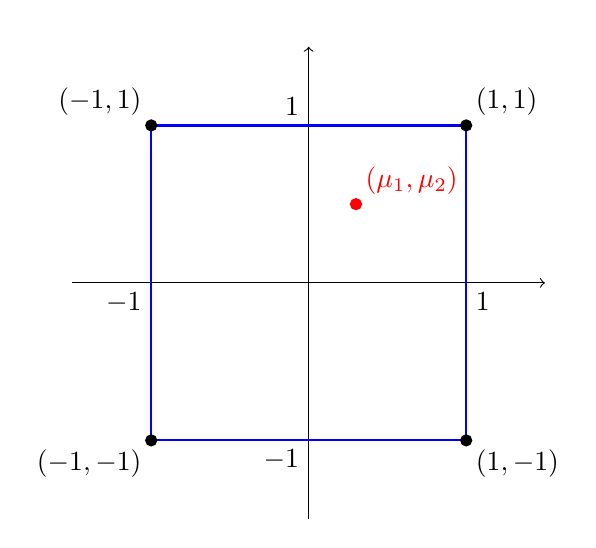
\begin{tikzpicture}[scale=2]
    % Axes
    \draw[->] (-1.5,0) -- (1.5,0) node[right] {};
    \draw[->] (0,-1.5) -- (0,1.5) node[above] {};

    % Carré
    \draw[thick, blue] (-1,-1) rectangle (1,1);

    % Points
    \filldraw (1,1) circle (1pt) node[above right] {$(1,1)$};
    \filldraw (-1,1) circle (1pt) node[above left] {$(-1,1)$};
    \filldraw (-1,-1) circle (1pt) node[below left] {$(-1,-1)$};
    \filldraw (1,-1) circle (1pt) node[below right] {$(1,-1)$};

    % Point intérieur
    \filldraw[red] (0.3,0.5) circle (1pt) node[above right, text=red] {$(\mu_1, \mu_2)$};

    % Labels axes
    \node[below right] at (1,0) {$1$};
    \node[below left] at (-1,0) {$-1$};
    \node[above left] at (0,1) {$1$};
    \node[below left] at (0,-1) {$-1$};
\end{tikzpicture}
\end{center}

\subsection{Calcul de distance dans \texorpdfstring{$\mathcal{M}_n(\R)$}{Mn(R)}}

On munit $\R^n$ de la norme euclidienne, et $\mathcal{M}_n(\R)$ de la norme subordonnée associée $\norm{M} = \sup_{\norm{x}=1} \norm{Mx}$.
On cherche à calculer la distance de la matrice nulle $0$ au sous-ensemble $SL_n(\R)$, c'est-à-dire $d(0, SL_n(\R))$.

Rappelons que $SL_n(\R) = \{ M \in \mathcal{M}_n(\R) \mid \det M = 1 \}$.
On cherche donc $d = \inf_{\det M = 1} \norm{M}$.

\lvspace \avspace \idee{Utiliser la décomposition polaire pour se ramener à l'étude des valeurs propres d'une matrice symétrique définie positive de déterminant 1.}

Soit $M \in SL_n(\R)$. Écrivons sa décomposition polaire $M = \Omega S$ avec $\Omega \in O_n(\R)$ et $S \in S_n^{++}(\R)$.
Puisque $\Omega$ est une isométrie, la norme subordonnée est invariante par multiplication orthogonale :
\[ \norm{M} = \norm{\Omega S} = \norm{S} \]
La matrice $S$ étant symétrique définie positive, sa norme subordonnée est égale à sa plus grande valeur propre $\lambda_{\text{max}}(S)$.
De plus, $\det M = \det(\Omega) \det(S)$. Or $\det(\Omega) = \pm 1$. Comme $\det(S) > 0$ (car $S \in S_n^{++}(\R)$) et $\det(M) = 1$, on a nécessairement $\det(\Omega) = 1$ et $\det(S) = 1$.
Le déterminant de $S$ est le produit de ses valeurs propres : $\prod_{i=1}^n \lambda_i = 1$.
Sachant que toutes les valeurs propres sont strictement positives, il est impossible que toutes soient strictement inférieures à 1 (sinon le produit le serait aussi).
Il existe donc au moins une valeur propre supérieure ou égale à 1, ce qui implique :
\[ \norm{M} = \lambda_{\text{max}}(S) \ge 1 \]
On a donc minoré la distance par 1.
De plus, pour la matrice identité $I_n$, on a $I_n \in SL_n(\R)$ et $\norm{I_n} = 1$.
Le minimum est donc atteint.
En conclusion, $d(0, SL_n(\R)) = 1$.

\section{Inégalité de convexité}

\begin{proposition}{}{}
    L'application $f : \begin{array}[t]{ccc}
    S_n^{++}(\R) & \to & \R \\
    S & \mapsto & (\det S)^{1/n}
    \end{array}$ est concave.
\end{proposition}

\lvspace \avspace \idee{Exprimer $(\det S)^{1/n}$ comme un infimum de fonctions linéaires en $S$ en utilisant l'inégalité arithmético-géométrique sur les valeurs propres d'un produit bien choisi.}
\begin{proof}
    Soient $S, H \in S_n^{++}(\R)$.
    La matrice $S H^{-1}$ est semblable à $H^{-1/2} S H^{-1/2}$, qui est symétrique définie positive.
    En effet : $H^{-1/2} (S H^{-1}) H^{1/2} = H^{-1/2} S H^{-1/2}$.
    Par conséquent, $\Sp(S H^{-1}) \subset \R_+^*$. Notons $\lambda_1, \dots, \lambda_n > 0$ ses valeurs propres.

    L'inégalité arithmético-géométrique appliquée à ces valeurs propres donne :
    \[ \left( \prod_{i=1}^n \lambda_i \right)^{1/n} \le \frac{1}{n} \sum_{i=1}^n \lambda_i \]
    Ce qui se traduit matriciellement par :
    \[ (\det(S H^{-1}))^{1/n} \le \frac{1}{n} \tr(S H^{-1}) \]
    Soit encore :
    \[ \frac{(\det S)^{1/n}}{(\det H)^{1/n}} \le \frac{1}{n} \tr(S H^{-1}) \]
    On a égalité si et seulement si toutes les valeurs propres sont égales, c'est-à-dire si $S H^{-1} = \alpha I_n$, soit $S = \alpha H$.
    En réécrivant cette inégalité, on obtient pour tout $H \in S_n^{++}(\R)$ :
    \[ (\det S)^{1/n} \le \frac{(\det H)^{1/n}}{n} \tr(S H^{-1}) \]
    Puisque le cas d'égalité est atteignable (par exemple en choisissant $H = S$), on peut écrire :
    \[ (\det S)^{1/n} = \inf_{H \in S_n^{++}(\R)} \frac{(\det H)^{1/n}}{n} \tr(S H^{-1}) \]

    Pour une matrice $H$ fixée, l'application $\varphi_H : S \mapsto \frac{(\det H)^{1/n}}{n} \tr(S H^{-1})$ est linéaire en $S$.
    Toute fonction linéaire est à la fois convexe et concave.
    Une propriété fondamentale de la concavité stipule que l'infimum d'une famille quelconque de fonctions concaves (pourvu qu'il soit bien défini et fini) est une fonction concave.
    Ainsi, $S \mapsto (\det S)^{1/n}$ est l'infimum d'une famille de fonctions linéaires, elle est donc concave sur $S_n^{++}(\R)$.
\end{proof}